% Author: Izaak Neutelings (September 2020)
\documentclass[border=3pt,tikz]{standalone}
\usepackage{amsmath}
\usepackage{tikz}
\usepackage{physics}
\usepackage{siunitx}
\usepackage[outline]{contour} % glow around text
\usetikzlibrary{angles,quotes} % for pic
\usetikzlibrary{calc}
\contourlength{1.3pt}

\tikzset{>=latex} % for LaTeX arrow head
\usepackage{xcolor}
\colorlet{veccol}{green!70!black}
\colorlet{pathcol}{blue!40!black}
\colorlet{xcol}{blue!70!black}
\colorlet{vcol}{green!70!black}
\colorlet{acol}{red!50!blue!80!black!80}
\colorlet{omcol}{vcol!60!black}
\colorlet{myblue}{blue!70!black}
\colorlet{myred}{red!70!black}
\tikzstyle{vector}=[->,very thick,xcol,line cap=round]
\tikzstyle{mydashed}=[dash pattern=on 2pt off 2pt]
\tikzstyle{mass}=[line width=0.6,red!30!black,fill=red!40!black!10,rounded corners=1,
                  top color=red!40!black!20,bottom color=red!40!black!10,shading angle=20]
\newcommand\rightAngle[4]{
  \pgfmathanglebetweenpoints{\pgfpointanchor{#2}{center}}{\pgfpointanchor{#3}{center}}
  \coordinate (tmpRA) at ($(#2)+(\pgfmathresult+45:#4)$);
  \draw[white,line width=0.6] ($(#2)!(tmpRA)!(#1)$) -- (tmpRA) -- ($(#2)!(tmpRA)!(#3)$);
  \draw[] ($(#2)!(tmpRA)!(#1)$) -- (tmpRA) -- ($(#2)!(tmpRA)!(#3)$);
}


\begin{document}



% EARTH
\contourlength{0.7pt}
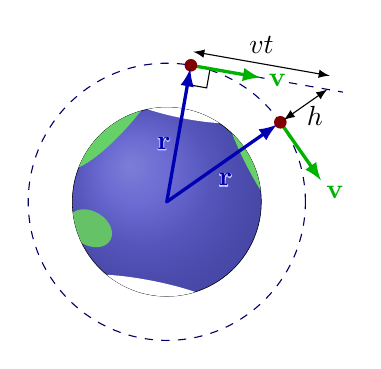
\begin{tikzpicture}
    \def\R{1.76}
    \def\anga{80}
    \def\angb{35}
    \def\E{1.2}
    \coordinate (O) at (0,0);
    \coordinate (A) at (\anga:\R);
    \coordinate (B) at (\angb:\R);
    \coordinate (H) at (\angb:{\R/cos(\anga-\angb)});
    \node[inner sep=1] (A') at (A) {};
    \node[inner sep=1] (B') at (B) {};

    % EARTH
    %\draw[dashed,rotate=-11] (0,-1.5*\E) -- (0,1.5*\E);
    \fill[blue!70!black!70] (0,0) circle (1.2);
    \draw[very thin,ball color=blue!70!black!40,fill opacity=0.3] (0,0) circle (\E);
    \begin{scope}[rotate=-11]
        \clip (0,0) circle (\E);
        \fill[white] (0,\E) ellipse ({0.6*\E} and {0.10*\E});
        \fill[white] (0,-\E) ellipse ({0.8*\E} and {0.15*\E});
        \fill[green!70!black!60,rotate=-30] (160:1.1*\E) ellipse ({0.2*\E} and {0.8*\E});
        \fill[green!70!black!60,rotate=40] (-10:1.14*\E) ellipse ({0.2*\E} and {0.9*\E});
        \fill[green!60!black!60,very thick,rotate=-20] % Australia
        (230:0.86*\E) ellipse ({0.25*\E} and {0.18*\E});
        %\draw[dashed] (-\E,0) -- (\E,0);
    \end{scope}

    % ORBIT
    \rightAngle{H}{A}{O}{0.35}
    \draw[pathcol,dashed] (O) circle (\R);
    \draw[pathcol,dashed] (A) -- (H) --++ (\anga-90:0.2);
    \draw[<->] (A)++(\anga:0.1*\R) --++ (\anga-90:{\R*tan(\anga-\angb)}) node[midway,above] {$vt$};
    \draw[vector,vcol]
    (A) --++ (\anga-90:0.9) node[scale=1,below=1,right=-1] {\contour{white}{$\vb{v}$}}; %,fill=white,inner sep=0] {$\vb{v}$}; 
    \draw[vector,vcol]
    (B) --++ (\angb-90:0.9) node[scale=1,below right=-2] {$\vb{v}$};
    \fill[red!50!black] (A) circle (0.08);
    \fill[red!50!black] (B) circle (0.08);
    \draw[<->] (H) -- (B') node[midway,below right=-3] {$h$};
    \draw[vector] (O) -- (A') node[midway,below=3,left=-1] {\contour{blue!20}{$\vb{r}$}};
    \draw[vector] (O) -- (B') node[midway,below=6,right=-5] {\contour{blue!20}{$\vb{r}$}};

\end{tikzpicture}

\end{document}